\documentclass{beamer}
\usepackage{amsmath,amssymb,latexsym,array,fancyheadings,mathdots}
\usepackage{algorithm,algorithmic}
\usepackage{hyperref}
\usepackage{color}
\usepackage{tabularx}
\usepackage[all]{xy}
\usepackage{qtree}
\usepackage{gitinfo2}

%% RCS
%\usepackage{rcs}

%% Colors
\definecolor{darkgreen}{rgb}{0,.4,0}
\definecolor{darkred}{rgb}{.5,0,0}
\definecolor{darkmagenta}{rgb}{.5,0,.5}
\definecolor{orange}{rgb}{1,.5,0}
\definecolor{lightblue}{rgb}{0.122,0.016,0.855}
\definecolor{darkocre}{rgb}{0.471,0.298,0.008}

\usetheme{default}

%% New Theorems
\newtheorem{thm}{Theorem}
\newtheorem{exm}[thm]{Example}
\newtheorem{cor}[thm]{Corollary}
\newtheorem{propo}[thm]{Proposition}
\newtheorem{lem}[thm]{Lemma}
\newtheorem{clm}[thm]{Claim}
\newtheorem{exr}[thm]{Exercise}
\newtheorem{dfn}[thm]{Definition}

%% New commands
\newcommand{\classfont}{\mathsf}
\newcommand{\ATM}{\classfont{A}_{\mathrm{TM}}}
\newcommand{\MTF}{\mathrm{MTF}}
\newcommand{\OPT}{\mathrm{OPT}}
\newcommand{\ALG}{\mathrm{ALG}}
\newcommand{\ALGNAIVE}{\mathrm{ALG}_{\text{na{\"\i}ve}}}
\newcommand{\LRU}{\mathrm{LRU}}
\newcommand{\FIFO}{\mathrm{FIFO}}
\newcommand{\FWF}{\mathrm{FWF}}
\newcommand{\LFD}{\mathrm{LFD}}
\newcommand{\true}{\mathsf{T}}
\newcommand{\false}{\mathsf{F}}
\newcommand{\also}{\wedge}
\newcommand{\lra}{\leftrightarrow}
\newcommand{\tc}{\textcolor}
\newcommand{\df}[1]{\textcolor{red}{\em #1}}
\newcommand{\highlight}[1]{\textcolor{orange}{\em #1}}
\newcommand{\hl}[1]{\textcolor{blue}{\em #1}}
\newcommand{\amp}{\texttt{\&}}
\newcommand{\hsh}{\texttt{\#}}
\newcommand{\ra}{\rightarrow}
\newcommand{\longra}{\longrightarrow}
\newcommand{\Ra}{\Rightarrow}
\newcommand{\rab}{{\rightarrow_\beta}}
\newcommand{\srab}{{\rightarrow^*_\beta}}
\newcommand{\aeq}{{=_\alpha}}
\newcommand{\order}{\mathrm{order}}
\newcommand{\rem}{\mathrm{rem}}
\newcommand{\IP}{\mathbf{IP}}
\newcommand{\PSPACE}{\mathbf{PSPACE}}
\newcommand{\thevalue}{\text{value}}
\newcommand{\pol}[1]{\mathbf{#1}}
\newcommand{\enc}{\text{Enc}}
\newcommand{\xor}{\oplus}
\newcommand{\zo}{\{0,1\}}
\newcommand{\SOPT}{S_{\mathrm{opt}}}
\newcommand{\la}{\leftarrow}
\newcommand{\myurl}[1]{\textcolor{darkgreen}{\url{#1}}}
\newcommand{\myhref}[2]{\textcolor{darkgreen}{\href{#1}{#2}}}
\newcommand{\qaccept}{q_{\mathrm{accept}}}
\newcommand{\qreject}{q_{\mathrm{reject}}}
\newcommand{\opt}{\text{\sc Opt}}
\newcommand{\tr}{\mathrm{tr}}
\newcommand{\csanky}{p^{\textsc{csanky}}}
\newcommand{\berk}{p^{\textsc{berk}}}

%% Algorithms package customization
\renewcommand{\algorithmicrequire}{\textbf{Pre-condition:}} 
\renewcommand{\algorithmicensure}{\textbf{Post-condition:}} 
\algsetup{indent=3em}

\input{prooftree}

%% including/excluding pauses
\newcommand{\ifpause}{\iftrue} % for including pauses
%\newcommand{\ifpause}{\iffalse} % for excluding pauses

%% 2nd or 3rd edition
\newif\ifthird
\thirdtrue
%\thirdfalse

%disables usefoottemplate
\setbeamertemplate{navigation symbols}{}
%\setbeamertemplate{footline}% 
%{\strut\quad\tiny 
%\begin{minipage}{3cm}
%Cryptography - Michael Soltys
%\today\ {\tt v\RCSRevision}
%\end{minipage}\hfill
%\insertsection\
%- \insertframenumber/\inserttotalframenumber\quad\strut}

\newcommand{\mytitle}{Computational Foundations \\ Appendix}
\newcommand{\mychpnr}{9}
%% Title page contents
\title{Intro to Analysis of Algorithms \\ \mytitle \\  Chapter \mychpnr}
\author{Michael Soltys}
\date{\textcolor{darkgreen}{\tiny\tt 
[ {\bf Git} Date:\gitAuthorDate\ 
Hash:\gitAbbrevHash\ 
Ed:\ifthird
3rd
\else
2nd
\fi]}}
\institute{CSU Channel Islands}

\setbeamertemplate{footline}{
  \colorbox{white}{\color{black}\tt
     \begin{tabularx}{0.97\textwidth}{XXX}
          IAA Chp \mychpnr\ - Michael Soltys \copyright & 
          \hfill\today\ (\gitAbbrevHash; \ifthird ed3\else ed2\fi)
					\hfill\phantom{.} & 
          \hfill\insertsection\ - \insertframenumber/\inserttotalframenumber \\
      \end{tabularx}}}

\begin{document}

\mode<presentation>
{
}

\parskip 8pt

\section{Introduction}

\begin{frame}
\titlepage
\end{frame}

\section{$\lambda$}

\begin{frame}
\begin{center}
\addtocounter{part}{1}
{\bf Part \Roman{part} \\ $\lambda$-calculus \\ (not in textbook)} 
\end{center}
\end{frame}

\begin{frame}

The set $\Lambda$ of \df{$\lambda$-terms} is the smallest set such
that:
\begin{itemize}
\item $x,y,z\ldots\in\Lambda$ (\df{variables} are in $\Lambda$)
\item if $x$ is a variable and $M$ is $\lambda$-term, then so is
$(\lambda x.M)$ (\df{abstraction})
\item if $M,N$ are $\lambda$-terms then so is $(MN)$
(\df{application})
\end{itemize}

$\text{FV}(M)$ is the set of free variables of $M$.  It is defined
recursively as follows: $\text{FV}(x)=\{x\}$, and $\text{FV}(\lambda
x.M)=\text{FV}(M)-\{x\}$ and
$\text{FV}(MN)=\text{FV}(M)\cup\text{FV}(N)$.

Terms without free variables are \df{closed terms} (also called
\df{combinators}), i.e., $M$ is closed iff $\text{FV}(M)=\emptyset$.

$\text{BV}(M)$ is the set of bounded variables of $M$.
$\text{BV}(x)=\emptyset$, $\text{BV}(\lambda
x.M)=\{x\}\cup\text{BV}(M)$ and $\text{BV}(M)\cup\text{BV}(N)$.
\end{frame}

\begin{frame}
Ex. $\lambda z.z$ is closed, and $\text{FV}(z\lambda x.x)=\{z\}$ while
$\text{BV}(z\lambda x.x)=\{x\}$.  On the other hand
$\text{BV}(x\lambda x.x)=\text{BV}(x\lambda x.x)=\{x\}$.

It is important to realize that two formulas are essentially the same
if they only differ in the names of bounded variables, e.g., $\lambda
x.x$ and $\lambda y.y$ represent (in some sense) the same object.  To
make this concept precise, we introduce the notion of
\df{$\alpha$-equality}, denoted $=_\alpha$.

$M\aeq N$ if $M=N=x$

Note that the equalith on the right ($M=N=x$) is {\em syntactic}
equality and $x$ can be any variable.

$M\aeq N$ if $M=M_1M_2$ and $N=N_1N_2$ and $M_1\aeq N_1$ and $M_2\aeq
N_2$.
\end{frame}

\begin{frame}
Also, $M\aeq N$ if $M=\lambda x.M_1$ and $N=\lambda x.N_1$ and
$M_1\aeq N_1$.

Finally, $M\aeq N$ if $M=\lambda x.M_1$ and $N=\lambda y.N_1$ and
there is a {\em new} variable $z$ such that $M_1\{x\mapsto z\}\aeq
N_1\{y\mapsto z\}$.

Here $M\{x\mapsto N\}$ denotes the $\lambda$-term $M$ where every {\em
free} instance of $x$ has been replaced by the $\lambda$-term $N$, in
such a way that no free variable $u$ of $N$ has been ``caught'' in the
scope of some $\lambda u$.  If $z$ is new, it will never be caught.

We shall soon give a formal definition of substitution.

But first: $\aeq$ is an equivalence relation.  

Ex. $\lambda x.x\aeq \lambda y.y$, $\lambda x.\lambda y.xy\aeq \lambda
z_1.\lambda z_2.z_1z_2$ and $(\lambda x.x)z\aeq(\lambda y.y)z$.

Thus, we think of $\lambda$-terms in terms of their equivalence
classes wrt $\aeq$ relation.
\end{frame}

\begin{frame}
We now define the notion of computation: a \df{redex} is a term of the
form $(\lambda x.M)N$.  The idea is to apply the function $\lambda
x.M$ to the argument $N$.  We do this as follows:
$$
(\lambda x.M)N\rab M\{x\mapsto N\}
$$
This is the so called \df{$\beta$-reduction} rule.  We write $M\rab
M'$ to indicate that $M$ reduces to $M'$.

Ex. $(\lambda x.x)y\rab x\{x\mapsto y\}=y$

(again, note that the equality is a syntactic equality)

$(\lambda x.\lambda y.x)(\lambda x.x)u
\rab(\lambda y.\lambda z.z)u
\rab\lambda z.z$

(application associates to the left, i.e., $MNP=(MN)P$)
\end{frame}

\begin{frame}
Ex. $(\lambda x.\lambda y.xy)(\lambda x.x)
\rab\lambda y.(\lambda x.x)y
\rab\lambda y.y$

The symbol $\srab$ means zero or more applications of $\rab$; from
the previous example,
$(\lambda x.\lambda y.xy)(\lambda x.x)\srab\lambda y.y$.

We use the word {\em reduce} but this does not mean that the terms
necessarily get simpler/smaller.

Ex. $(\lambda x.xx)(\lambda xyz.xz(yz))
\rab(\lambda xyz.xz(yz))(\lambda xyz.xz(yz))$

(note that $\lambda xyz$ abbreviates $\lambda x.\lambda y.\lambda z$,
and that abstractions associate to the right, i.e., $\lambda xyz.M$ is
$\lambda x.(\lambda y.(\lambda z.M))$)
\end{frame}

\begin{frame}
\begin{align*}
(\lambda x.xx)(\lambda y.yx)z & = ((\lambda x.xx)(\lambda y.yx))z
\tag*{[application left associates]} \\
&\rab ((xx)\{x\mapsto (\lambda y.yx)\})z 
\tag*{[substitution]} \\
&= ((\lambda y.yx)(\lambda y.yx))z \\
&\rab ((yx)\{y\mapsto (\lambda y.yx)\})z
\tag*{[substitution]} \\
&= ((\lambda y.yx)x)z \\
&\rab ((yx)\{y\mapsto x\})z
\tag*{[substitution]} \\
&= (xx)z = xxz
\tag*{[application left associates]}
\end{align*}

\begin{align*}
(\lambda x.(\lambda y.(xy))y)z
&\rab (\lambda x.((xy)\{y\mapsto y\}))z \\
&= (\lambda x.(xy))z \\
&\rab (xy)\{x\mapsto z\}=zy
\end{align*}
\end{frame}

\begin{frame}
\begin{align*}
((\lambda x.xx)(\lambda y.y))(\lambda y.y)
&\rab ((xx)\{x\mapsto (\lambda y.y)\})(\lambda y.y) \\
&=((\lambda y.y)(\lambda y.y))(\lambda y.y) \\
&\rab (y\{y\mapsto(\lambda y.y)\})(\lambda y.y) \\
&=(\lambda y.y)(\lambda y.y) \\
&=(\lambda y.y)
\tag*{[just repeating previous line]}
\end{align*}

\begin{align*}
(((\lambda x.\lambda y(xy))(\lambda y.y))w)
&= (((\lambda x.\lambda v.(xv))(\lambda y.y))w)
\tag*{[use $=_\alpha$ so $y$ not ``caught'' by $\lambda y$]} \\
&\rab ((\lambda v.(xv))\{x\mapsto(\lambda y.y)\})w \\
&= (\lambda v.((\lambda y.y)v))w \\
&\rab (\lambda v.v)w \\
&\rab w
\end{align*}
\end{frame}

\begin{frame}
We now give a precise definition of \df{substitution} $M\{x\mapsto N\}$
by structural induction on $M$.

$x\{x\mapsto N\}N=N$

$y\{x\mapsto N\}=y$

$(PQ)\{x\mapsto N\}=(P\{x\mapsto N\})(Q\{x\mapsto N\})$

$(\lambda x.P)\{x\mapsto N\}=\lambda x.P$

$(\lambda y.P)\{x\mapsto N\}=\lambda y.(P\{x\mapsto N\})$ if
$y\notin\text{FV}(N)$ or $x\notin\text{FV}(P)$

$(\lambda y.P)\{x\mapsto N\}=(\lambda z.P\{y\mapsto z\})\{x\mapsto
N\}$ otherwise and $z$ is a new variable
\end{frame}

\begin{frame}
Ex.
\begin{align*}
(\lambda z.yz)\{y\mapsto z\} 
&\aeq (\lambda x.(yz)\{z\mapsto x\})\{y\mapsto z\} \\
&\aeq (\lambda x.((y\{z\mapsto x\})(z\{z\mapsto x\})))\{y\mapsto z\} \\
&\aeq (\lambda x.(yx))\{y\mapsto z\} \\
&\aeq \lambda x.(yx)\{y\mapsto z\} \\
&\aeq \lambda x.((y\{y\mapsto z\})(x\{y\mapsto z\})) \\
&\aeq \lambda x.(zy)
\end{align*}

{\bf Property:} If $x\in\text{FV}(P)$, then
$$
(M\{x\mapsto N\})\{y\mapsto P\}\aeq
(M\{y\mapsto P\})\{x\mapsto N\{y\mapsto P\}\}
$$
\end{frame}

\begin{frame}
A \df{normal form} is a term that does not contain any redexes.

A term that can be reduced to normal form is called \df{normalizable}.

Ex. $\lambda abc.((\lambda x.a(\lambda y.xy))bc)\rab
\lambda abc.(a(\lambda y.by)c)$ where the last term is in normal form
(bec applications associate to the left)

Some terms are not normalizable, e.g., $(\lambda x.xx)(\lambda x.xx)$.

A term $M$ is \df{strongly normalizable} (or \df{terminating}) if all
reduction sequences starting from $M$ are finite.

\df{Weak head normal form}: stop reducing when there are no redexe
left, but without reducing under an abstraction.

Ex. $\lambda abc.((\lambda x.a(\lambda xy))bc)$ is in weak head normal
form.
\end{frame}

\begin{frame}

{\bf FACT:} Our reduction relation $\rab$ is \df{confluent} because
whenever $M\rab M_1$ and $M\rab M_2$, then there exists a term $M_3$
such that $M_1\rab M_3$ and $M_2\rab M_3$.

{\bf Corollary:} Each $\lambda$-term has at most one normal form.

{\bf Proof:} Suppose that a term $M$ has more than one normal form;
i.e., $M\rightarrow^*_\beta M_1$ and $M\rightarrow^*_\beta M_2$, where
$M_1$ and $M_2$ are in normal form.  Then they should both be
reducible to a common $M_3$ (by confluence), but if they are in normal
form that cannot be done.  Contradiction---hence there can be at most
one normal form.

\end{frame}

\begin{frame}

\df{Church's numerals}:

\begin{align*}
\bar{0} &= \lambda x.\lambda y.y \\
\bar{1} &= \lambda x.\lambda y.xy \\
\bar{2} &= \lambda x.\lambda y.x(xy) \\
\bar{3} &= \lambda x.\lambda y.x(x(xy)) \\
        &\vdots \\
\bar{n} &= \lambda x.\lambda y.\underbrace{x(x(x\ldots(x}_{n}y)\ldots)) \\
        &\vdots
\end{align*}
\end{frame}

\begin{frame}
\begin{minipage}{5cm}
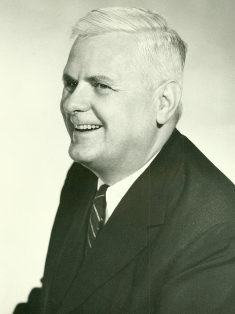
\includegraphics[width=4cm]{figures/AlonzoChurch.jpg}
\end{minipage}
\begin{minipage}{5cm}
\myhref{http://en.wikipedia.org/wiki/Alonzo_Church}{Alonzo Church} \\
\end{minipage}
\end{frame}

\begin{frame}
Consider $S:=\lambda xyz.y(xyz)$
\begin{align*}
S\bar{n} &= S(\lambda xy\underbrace{x(x(x\ldots(x}_{n}y)\ldots))) \\
&\rab \lambda yz.y(\lambda xy.\underbrace{x(x(x\ldots(x}_{n}y)\ldots))yz) \\
&\aeq \lambda yz.y(\lambda xw.\underbrace{x(x(x\ldots(x}_{n}w)\ldots))yz) \\
&\rab \lambda yz.y(\lambda w.\underbrace{y(y(y\ldots(y}_{n}w)\ldots))z) \\
&\rab \lambda yz.\overbrace{y(\underbrace{y(y(y\ldots(y}_{n}}^{n+1}z)
\ldots))) \aeq \overline{n+1}
\end{align*}
so $S(\bar{n})=\overline{n+1}$, i.e., $S$ is the successor fn.
\end{frame}

\begin{frame}

Define $\text{ADD}:=\lambda xyab.(xa)(yab)$.

\begin{align*}
\text{ADD}\bar{n}\bar{m}
&\rab (\lambda yab.(\bar{n}a)(yab))\bar{m} \\
&\rab \lambda ab.(\text{\colorbox{yellow}{$\bar{n}a$}})
(\text{\colorbox{orange}{$\bar{m}a$}}b) \\
&\rab \lambda ab.(
\text{\colorbox{yellow}{$\lambda
y\underbrace{a(a(a\ldots(a}_{n}y)\ldots))$}})
[(\text{\colorbox{orange}{$\lambda
y\underbrace{a(a(a\ldots(a}_{m}y)\ldots))$}})b] \\
&\rab \lambda ab.(
\text{\colorbox{yellow}{$\lambda
y\underbrace{a(a(a\ldots(a}_{n}y)\ldots))$}})
[\text{\colorbox{green}{$\underbrace{a(a(a\ldots(a}_{m}b)\ldots))$}}] \\
&\rab \lambda ab.(\underbrace{\underbrace{a(a(\ldots(a}_{n}
\underbrace{(a(a\ldots(a}_{m}}_{n+m}b)\ldots)))\ldots))) \\
&\aeq\overline{n+m}
\end{align*}
\end{frame}

\section{RFs}

\begin{frame}
\begin{center}
\addtocounter{part}{1}
{\bf Part \Roman{part} \\ Recursive Functions \\ (not in textbook)} 
\end{center}
\end{frame}

\begin{frame}

A \df{partial function} is a function
$$
f:(\mathbb{N}\cup\{\infty\})^n\longrightarrow
\mathbb{N}\cup\{\infty\}, \quad n\ge 0
$$
such that $f(c_1,\ldots,c_n)=\infty$ if some $c_i=\infty$.

$\text{Domain}(f)=\{\vec{x}\in\mathbb{N}^n:f(\vec{x})\neq\infty\}$
where $\vec{x}=(x_1,\ldots,x_n)$.

$f$ is \df{total} if $\text{Domain}(f)=\mathbb{N}^n$, i.e., $f$ is
always defined if its arguments are defined.
\end{frame}

\begin{frame}

A \df{Register Machine (RM)} is a computational model specified by a
program $P=\langle c_0,c_1,\ldots,c_{h-1}\rangle$, consisting of a
finite sequence of commands.

The commands operate on registers $R_1,R_2,R_3,\ldots$, each capable
of storing an arbitrary natural number.

\bigskip

\begin{tabular}{l|c|l}
command & abbrev. & parameters \\\hline
$R_i\leftarrow 0$ & $Z_i$ & $i=1,2,\ldots$ \\
$R_i\leftarrow R_i+1$ & $S_i$ & $i=1,2,\ldots$ \\
goto $k$ if $R_i=R_j$ & $J_{ijk}$ & $i,j=1,2,\ldots$ \amp\
$k=0,1,2,\ldots h$
\end{tabular}
\end{frame}

\begin{frame}
An example RM program that copies $R_i$ into $R_j$:

\begin{tabular}{lll}
$c_0$: & $R_j\leftarrow 0$ & $Z_j$ \\
$c_1$: & goto 4 if $R_i=R_j$ & $J_{ij4}$ \\
$c_2$: & $R_j\leftarrow R_j+1$ & $S_j$ \\
$c_3$: & goto 1 if $R_1=R_1$ & $J_{111}$ \\
$c_4$:
\end{tabular}

Formally, the program is $\langle Z_j,J_{ij4},S_j,J_{111}\rangle$.
\end{frame}

\begin{frame}

{\bf Semantics of RM's}

A \df{state} is an $m+1$-tuple
$$
\langle K,R_1,\ldots,R_m\rangle
$$
of natural numbers, where $K$ is the instruction counter (i.e., the
number of the next command to be executed), and $R_1,\ldots,R_m$ are
the current values of the registers ($m$ is the max
register index referred to in the program).

Given a state $s=\langle K,R_1,\ldots,R_m\rangle$ and a program
$P=\langle c_0,c_1,\ldots,c_{h-1}\rangle$, the next state,
$s'=\text{Next}_P(s)$ is the state resulting when command $c_K$ is
applied to the register values given by $s$.

We say that $s$ is a \df{halting state} if $K=h$, and in this case
$s'=s$.
\end{frame}

\begin{frame}
Suppose the state $s=\langle K,R_1,\ldots,R_m\rangle$ and the command
$c_k$ is $S_j$, where $1\le j\le m$.  Then,
$$
\text{Next}_P(s)=\langle
K+1,R_1,\ldots,R_{j-1},R_j+1,R_{j+1},\ldots,R_m\rangle
$$

Ex. Give a formal definition of the function $\text{Next}_P$ for the cases
in which $c_K$ is $Z_i$ and $J_{ijk}$.
\end{frame}

\begin{frame}
A computation of a program $P$ is a finite or infinite sequence
$s_0,s_1,\ldots$ of states such that $s_{i+1}=\text{Next}_P(s_i)$. 

If the sequence is finite, then the last state must be a halting
state, in which case that computation is halting---we say that $P$ is
halting starting in state $s_0$.

A program $P$ computes a (partial) function $f(a_1,\ldots,a_n)$ as
follows.  Initially place $a_1,\ldots,a_n$ in $R_1,\ldots,R_n$ and set
all other registers to 0.  Start execution with $c_0$, i.e., the
initial state is
$$
s_0=\langle 0,a_1,\ldots,a_n,0,\ldots,0\rangle
$$
If $P$ halts in $s_0$, the final value of $R_1$ must be
$f(a_1,\ldots,a_n)$ (which then must be defined).  If $P$ fails to
halt, then $f(a_1,\ldots,a_n)=\infty$.
\end{frame}

\begin{frame}
We say $f$ is \df{RM-computable} (or just \df{computable}) if $f$ is
computed by some RM program.

{\bf Church's Thesis:}  Every algorithmically computable function is
RM computable.

Ex. Show $P=\langle J_{234},S_1,S_3,J_{110}\rangle$ computes $f(x,y)=x+y$.

Ex. Write RM programs that compute $f_1(x)=x\stackrel{.}{-}1$ and
$f_2(x,y)=x\cdot y$.  Be sure to respect the input/output conventions
for RMs.
\end{frame}

\begin{frame}
$f$ is defined from $g$ and $h$ by \df{primitive recursion (pr)} if
\begin{align*}
& f(\vec{x},0)=g(\vec{x}) \\
& f(\vec{x},y+1)=h(\vec{x},y,f(\vec{x},y))
\end{align*}
we allow $n=0$ so $\vec{x}$ could be missing.
The following high-level program computes $f$ from $g,h$ by
pr:
\begin{tabbing}
$u\leftarrow g(\vec{x})$ \\
for \= $z:0\ldots(y-1)$ \\
    \> $u\leftarrow h(\vec{x},z,u)$ \\
end for
\end{tabbing}

$f_+(x,y)=x+y$ can be define by pr as follows:
\begin{align*}
& x+0=x \\
& x+(y+1)=(x+y)+1
\end{align*}
In this case $g(x)=x$ and $h(x,y,z)=z+1$.
\end{frame}

\begin{frame}
$f$ is defined from $g$ and $h_1,\ldots,h_m$ by \df{composition} if
$f(\vec{x})=g(h_1(\vec{x}),\ldots,h_m(\vec{x}))$, where
$f,h_1,\ldots,h_m$ are each $n$-ary and $g$ is $m$-ary.

\df{Initial functions:}
\begin{tabular}{ll}
$Z$ & $0$-ary constant function equal to 0 \\
$S$ & $S(x)=x+1$ \\
$\pi_{n,i}(x_1,\ldots,x_n)=x_i$ & infinite class of \df{projection}
functions
\end{tabular}

$f$ is \df{primitive recursive (pr)} if $f$ can be obtained from the
initial functions by finitely many applications of primitive recursion
and composition.

{\bf Proposition:} Every pr function is total.
\end{frame}

\begin{frame}

{\bf Theorem:} Every pr function is RM-computable.

{\bf Proof:} We show every pr $f$ is computable by a program which
upon halting leaves all registers 0 except $R_1$ (which contains the
output).  We do this by induction on the def of pr fns.

Base case: each initial fn is computable by such an RM program.

$Z$ is just $\langle Z_1\rangle$ \\
$S(x)=x+1$ is $\langle S_1\rangle$ \\
$\pi_{n,i}(x_1,\ldots,x_n)$ depends on whether $i=1$ or $i\neq 1$.  In
the first case the program is $\langle Z_2,\ldots,Z_n\rangle$.  In the
second case it is $\langle
\underbrace{Z_1,J_{i14},S_1,J_{111}}_\text{``Copy $R_i$ to
$R_1$''},Z_2,\ldots,Z_n\rangle$.
\end{frame}

\begin{frame}
Induction step:  
Composition: Assume that $g,h_1,\ldots,h_m$ are computable by programs
$P_g,P_{h_1},\ldots,P_{h_m}$, where these programs leave all registers
zero except $R_1$.

We must show that $f$ is computable by a program $P_f$ where
$f(\vec{x})=g(h_1(\vec{x}),\ldots,h_m(\vec{x}))$.  At the start
$\vec{x}=x_1,\ldots,x_n$ are in registers $R_1,\ldots,R_n$, with all
other registers zero.

Program $P_f$ must proceed (at a high level) as follows: it must move
$\vec{x}$ out of the way, to some high-numbered registers.  Then it
must compute $h_i(\vec{x})$, for each $i$, by moving a $\vec{x}$ to
$R_1,\ldots, R_n$, simulating $P_{h_i}$, and then moving the result
from $R_1$ out of the way.

At the end it must move the value of $h_i(\vec{x})$ to $R_i$, for each
$i$, and simulate $P_g$.

Primitive recursion: implement the high-level program given following
the definition of pr.
\end{frame}

\begin{frame}
Is the converse true?  Is every computable fn pr?

No.  Some computable fns are not total.

Is every total computable fn pr?

No.  We can show this by a diagonal argument: each pr fn can be
encoded as a number; let $f_1,f_2,f_3,\ldots$ be the list of all pr
functions.

We are only interested in unary fns, so if $f_i$ has arity greater
than one, we replace it by $S$ (the unary successor function).  Let
the new list be $g_1,g_2,g_3,\ldots$, where $g_i=f_i$ if $f_i$ was
unary, and $g_i=S$ otherwise.

Let $U(x,y)=g_x(y)$, so $U$ is a total computable fn.  However, $U$ is
not pr; for suppose that it is.  Then so is $D(x)=S(U(x,x))$.  If $U$
were pr, so would be $D$.  

But if $D$ is pr, then $D=g_e$ for some $e$.  This gives us a
contradiction, since $g_e(e)=D(e)=g_e(e)+1$.
\end{frame}

\begin{frame}
We can in fact give a concrete example of a total computable fn, which
is not primitive recursive. 

The \df{Ackermann function} is defined as follows:
$$
A_0(x)=\begin{cases}
x+1 & \text{if $x=0$ or $x=1$} \\
x+2 & \text{otherwise}
\end{cases}
$$
and $A_{n+1}(0)=1$ and $A_{n+1}(x+1)=A_n(A_{n+1}(x))$.

We can prove by induction on $n$ that $A_n(x)$ is total for all $n$,
and therefore so is $A(n,x)=A_n(x)$.  Also, $A$ is computable since it
can be computed with an RM program following the recursion given
above.

Note that $A_2(x)=2^x$ while
$A_3(x)=\left. 2^{2^{2^{\iddots^2}}}\right\}$ of height
$x$.
\end{frame}

\begin{frame}

{\bf Lemma:} For each $n$, $A_n$ is pr.

{\bf Proof:} By induction on $n$; the work is in the base case.

{\bf Fact:}  For every pr fn $h(\vec{x})$, there exists an $n$ so that
for sufficiently large $B$, if $\min\{\vec{x}\}>B$ then
$h(\vec{x})<A_n(\max\{\vec{x}\})$, i.e., $A_n$ dominates $h$.  

Then, if $A(n,x)=A_n(x)$, then $A$ is not pr; in fact, $F(x)=A(x,x)$
is not pr, since $A$ cannot dominate itself.


\end{frame}

\begin{frame}
We let $\mu$ denote the least number operator.  More precisely,
$f(\vec{x})=\mu y[g(\vec{x},y)=0]$ if
\begin{enumerate}
\item  $f(\vec{x})$ is the least number $b$ such that
$g(\vec{x},b)=0$,
\item  $g(\vec{x},y)\neq\infty$ for $i<b$.
\end{enumerate}
$f(\vec{x})=\infty$ if no such $b$ exists.

If $g$ is computable and $f(\vec{x})=\mu y[g(\vec{x},y)=0]$ then $f$
is also computable:

\begin{tabbing}
for \= $y=0\ldots\infty$ \\
    \> if \= $g(\vec{x},y)=0$ then \\
    \>    \> output $y$ and exit \\
    \> end if \\
end for
\end{tabbing}
\end{frame}

\begin{frame}
A function $f$ is \df{recursive} if $f$ can be obtained from the
initial functions by finitely many applications of composition,
primitive recursion, and minimization.

{\bf Theorem:} Every recursive function is computable.

In the 1940s Kleene showed that the converse of the above theorem is
also true: every computable function is recursive.

We next prove this converse: every computable fn is recursive.
\end{frame}

\begin{frame}
First we assign a \df{G{\"o}del number} $\hsh P$ to every program
$P$:

\begin{tabular}{l|c|c|c}
command $c$ & $Z_i$ & $S_i$ & $J_{ijm}$ \\\hline
&&& \\
code    $\hsh c$ & $2^i$ & $3^i$ & $5^i7^j11^m$
\end{tabular}

By the {\bf Fundamental Theorem of Arithmetic} these codes are unique.

Let $p_0<p_1<p_2<\cdots=2<3<5<\cdots$ be the list of all primes, in
order.  Then, if $P=\langle c_0,c_1,\ldots,c_{h-1}\rangle$,
$$
\hsh P=p_0^{\hsh c_0}p_1^{\hsh c_1}\cdots p_{h-1}^{\hsh c_{h-1}}
$$

Encode the state $s$ of a program as follows:
$$
\hsh s=\hsh\langle K,R_1,\ldots,R_m\rangle
=p_0^kp_1^{R_1}\cdots p_m^{R_m}
$$
\end{frame}

\begin{frame}
\begin{minipage}{5cm}
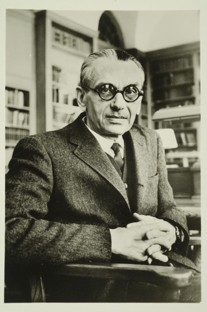
\includegraphics[width=4cm]{figures/KurtGodel.jpg}
\end{minipage}
\begin{minipage}{5cm}
\myhref{http://en.wikipedia.org/wiki/Kurt_Godel}{Kurt G{\"o}del} \\
\end{minipage}
\end{frame}

\begin{frame}
\begin{minipage}{5cm}
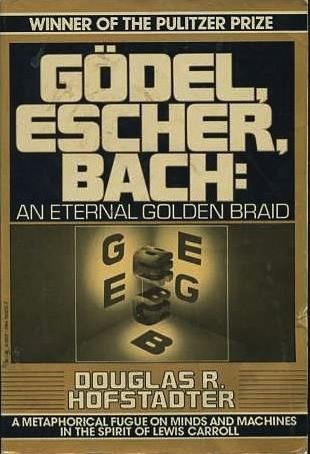
\includegraphics[width=4cm]{figures/geb.jpg}
\end{minipage}
\begin{minipage}{5cm}
G{\"o}del, Escher, Bach \\
\end{minipage}
\end{frame}

\begin{frame}
\begin{minipage}{5cm}
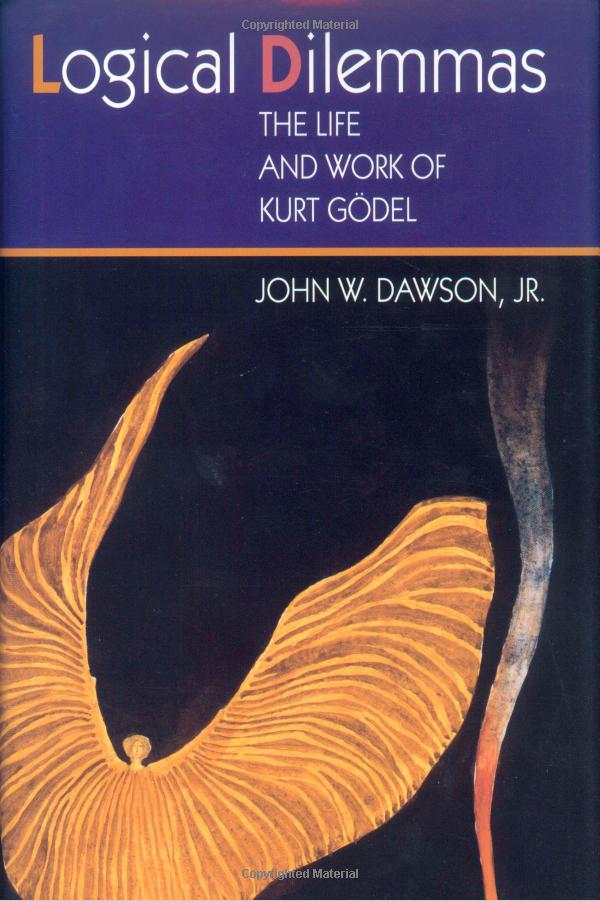
\includegraphics[width=4cm]{figures/logicaldilemmas.png}
\end{minipage}
\begin{minipage}{5cm}
A serious study of G{\"o}del \\
\end{minipage}
\end{frame}

\begin{frame}
\begin{minipage}{5cm}
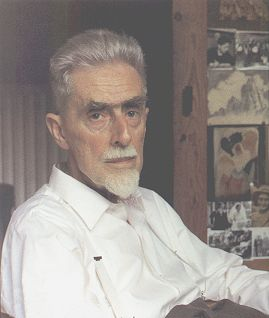
\includegraphics[width=4cm]{figures/escher_photo.jpg}
\end{minipage}
\begin{minipage}{5cm}
\myhref{http://en.wikipedia.org/wiki/M._C._Escher}{Maurits Escher} \\
\end{minipage}
\end{frame}

\begin{frame}
\begin{center}
\begin{minipage}{8cm}
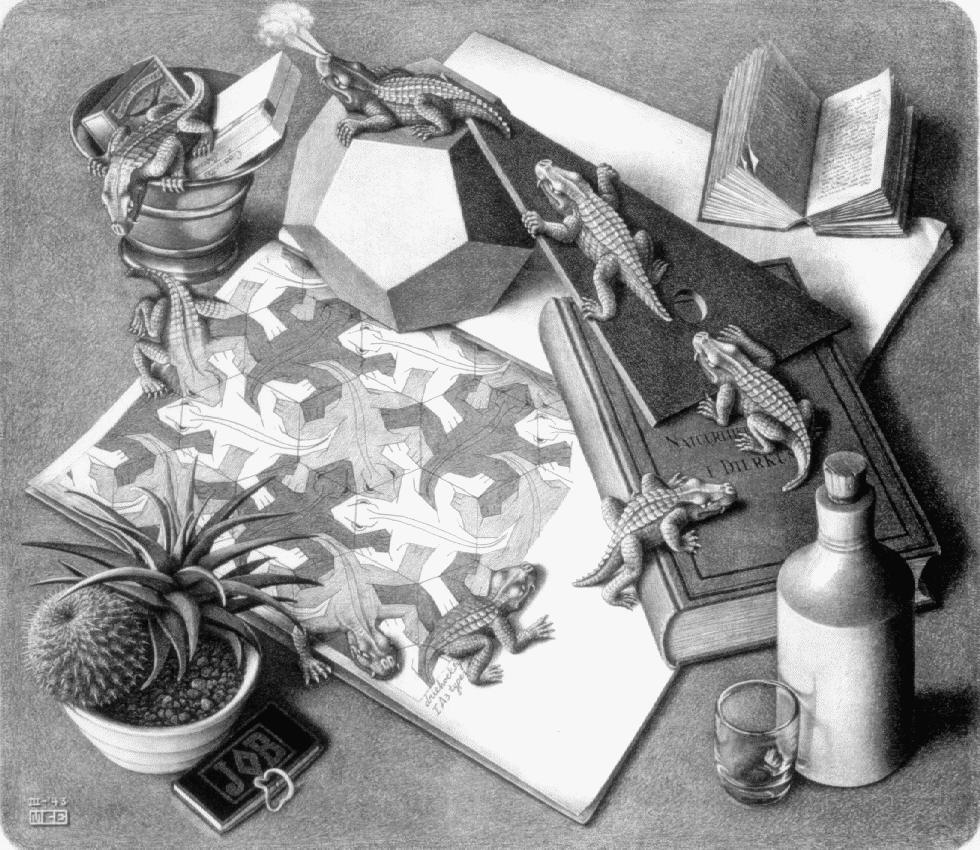
\includegraphics[width=8cm]{figures/escher1.jpg}
\end{minipage}
\end{center}
\end{frame}

\begin{frame}
\begin{center}
\begin{minipage}{6cm}
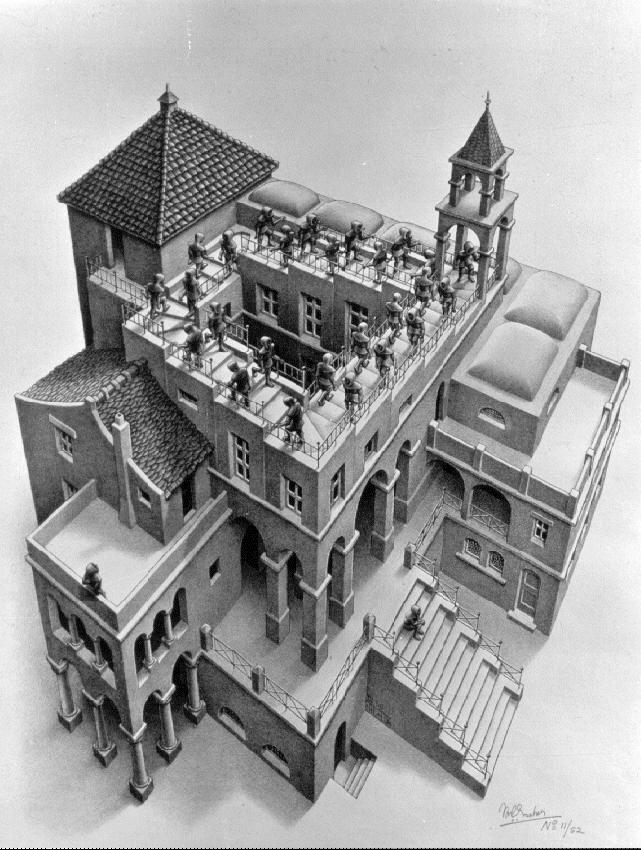
\includegraphics[width=6cm]{figures/escher2.jpg}
\end{minipage}
\end{center}
\end{frame}

\begin{frame}
\begin{center}
\begin{minipage}{6cm}
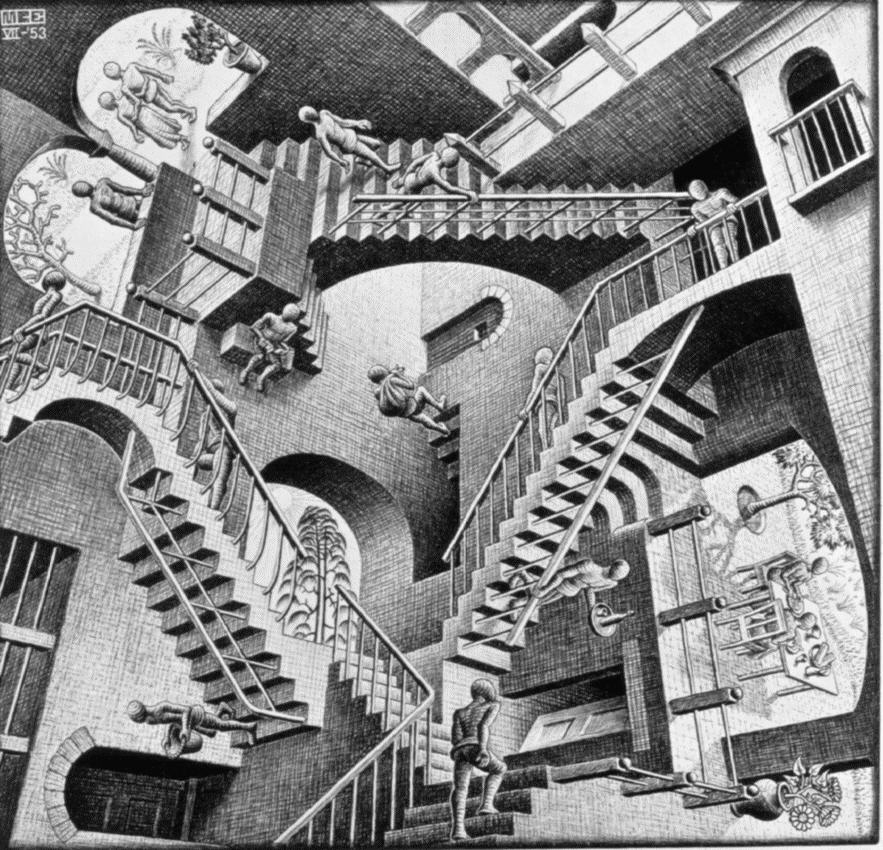
\includegraphics[width=6cm]{figures/escher3.jpg}
\end{minipage}
\end{center}
\end{frame}

\begin{frame}
\begin{center}
\begin{minipage}{6cm}
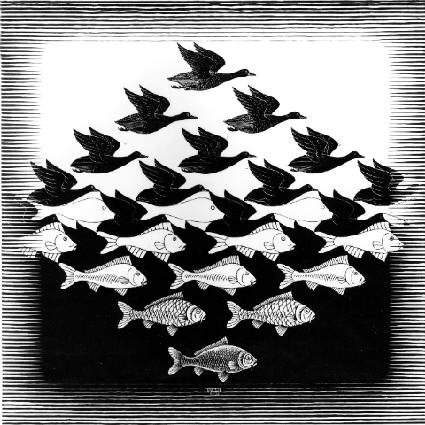
\includegraphics[width=6cm]{figures/escher4.jpg}
\end{minipage}
\end{center}
\end{frame}

\begin{frame}
\begin{center}
\begin{minipage}{8cm}
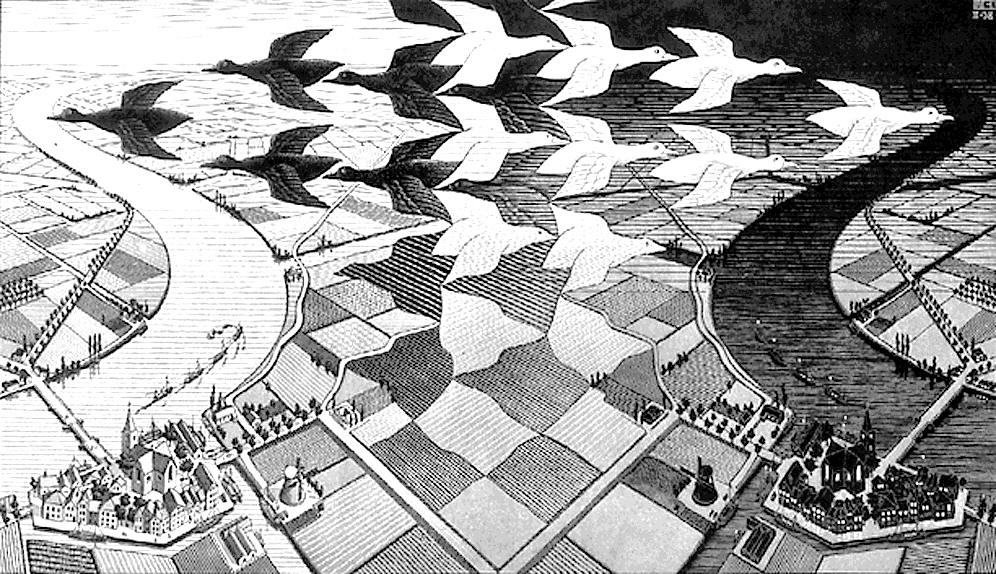
\includegraphics[width=8cm]{figures/escher5.jpg}
\end{minipage}
\end{center}
\end{frame}


\begin{frame}
Ex.  
\begin{align*}
& \hsh S_1=3^1=3 \\
& \hsh \langle S_1\rangle=2^{\hsh S_3}=2^3=8 \\
& \hsh \langle Z_1,S_1,J_{111}\rangle=2^{\hsh Z_1}\cdot
3^{\hsh S_1}\cdot 5^{\hsh J_{111}}=
2^{2^1}\cdot 3^{3^1}\cdot 5^{(5^17^111^1)}=4\cdot 27\cdot 5^{385}
\end{align*}

Distinct programs get distinct codes, and given a code we can extract
the (unique) program encoded by it \\
(or decide that it is not a code
for any program).

Ex. Given the number $10871635968$ we decompose it (uniquely) as a
product of primes:
$$
10871635968
=2^{27}\cdot 3^{4}
=2^{3^3}\cdot 3^{2^2}
=2^{\hsh \textcolor{red}{S_3}}\cdot 3^{\hsh \textcolor{red}{Z_2}}
=\hsh\langle \textcolor{red}{S_3},\textcolor{red}{Z_2}\rangle
$$
\end{frame}

\begin{frame}
We let $\text{Prog}(z)$ be a predicate that is true iff $z$ is the
code of some program $P$.  $\text{Prog}(z)$ is a pr predicate.

%We let $\hat{z}$ be $z$ if $\text{Prog}(z)$ is true, and 1 otherwise.

We let 
$$
\{z\}=\begin{cases}
\text{program $P$ such that $z=\hsh P$} & \text{if $P$ exists} \\
\text{the empty program $\langle\rangle$} & \text{otherwise}
\end{cases}
$$

The function $\text{Nex}(u,z)=u'$ is defined as follows: $u'$ is the
state resulting from a single step of $\{z\}$ on state $u$.  Nex is
pr.
\end{frame}

\begin{frame}
If $u_0,u_1,\ldots,u_t$ is the sequence of codes for the successive
states in a computation, then we code the entire computation by the
number $y=p_0^{u_0}p_1^{u_1}\cdots p_t^{u_t}$.  

\df{Kleene $T$ predicate:} for each $n\ge 1$ we define the $n+2$-ary
relation $T_n$ as follows: $T_n(z,\vec{x},y)$ is true iff $y$ codes
the computation of $\{z\}$ on input $\vec{x}$.  

{\bf Theorem:} For each $n\ge 1$, $T_n$ is pr.

Let $\{z\}_n$ be the $n$-ary fn computed by program $\{z\}$.

\colorbox{yellow}{\bf Kleene Normal Form Theorem:}  
There is a pr fn $U$ such that
$$
\forall n\ge 1,\qquad
\{z\}_n(\vec{x})=U(\mu yT_n(z,\vec{x},y))
$$
($U(y)$ extracts the contents of the first register in the last state
of computation $y$.)  Thus, every computable fn is recursive.
\end{frame}

\begin{frame}
\begin{center}
\addtocounter{part}{1}
{\bf Part \Roman{part} \\ CONCLUSION}
\end{center}
\end{frame}

\begin{frame}

{\bf Church-Turing thesis:} the following models of computation are
all equivalent:

\begin{itemize}
\item  Rewriting systems
\item  Turing machines
\item  $\lambda$-calculus
\item  Recursive functions
\item  Register machines
\item  \textcolor{darkmagenta}{\bf ZFC-computable}
\end{itemize}

Even more evidence that we have captures the notion of compation: ZFC
is the Zarmelo-Fraenkel set theory together with the Axiom of Choice.
All of mathematics can be formalized in ZFC.

A language $L$ is ZFC-computable if there exists a formula
$\alpha(x)$ such that if $w\in L\Rightarrow\text{ZFC}\vdash\alpha(w)$
and if $w\not\in L\Rightarrow\text{ZFC}\vdash\neg\alpha(w)$.
\end{frame}

\end{document}
